\documentclass[nochap]{apuntes}

\title{Métodos Numéricos para EDP}
\author{Guillermo Ruiz Álvarez}
\date{15/16 C1}

\setcounter{secnumdepth}{5}
\setcounter{tocdepth}{4} 
% Paquetes adicionales

% This is the color used for MATLAB comments below
\definecolor{MyDarkGreen}{rgb}{0.0,0.4,0.0}

% For faster processing, load Matlab syntax for listings
\lstloadlanguages{Matlab}
\lstset{language=Matlab,
	frame=single,                           % Single frame around code
	basicstyle=\footnotesize\ttfamily,      % Use small true type font
	keywordstyle=[1]\color{Blue}\bfseries,  % MATLAB functions bold and blue
	keywordstyle=[2]\color{Purple},         % MATLAB function arguments purple
	keywordstyle=[3]\color{Blue}\underbar,  % User functions underlined and blue
	identifierstyle=,                       % Nothing special about identifiers
	% Comments small dark green courier
	commentstyle=\usefont{T1}{pcr}{m}{sl}\color{MyDarkGreen}\small,
	stringstyle=\color{Purple},             % Strings are purple
	showstringspaces=false,                 % Don't put marks in string spaces
	tabsize=4,                              % 5 spaces per tab
	morecomment=[l][\color{Blue}]{...},     % Line continuation (...) like blue comment
	numbers=left,                           % Line numbers on left
	firstnumber=1,                          % Line numbers start with line 1
	numberstyle=\tiny\color{Blue},          % Line numbers are blue
	stepnumber=1                            % Line numbers go in steps of 5
}


% --------------------

\begin{document}
\pagestyle{plain}
\maketitle

\tableofcontents
\newpage
% Contenido.
\section{Métodos en diferencias finitas}
En esta sección vamos a ver métodos en diferencias finitas para distintos tipos de ecuaciones. Estos métodos se utilizan para calcular las soluciones aproximadas a las ecuaciones diferenciales aproximando derivadas.

\subsection{Ecuaciones parabólicas en una dimensión espacial.}
Este tipo de ecuaciones tiene la forma:
$$e(x,t)u_t = \underbrace{\frac{\partial}{\partial x} \left(a(x,t)\frac{\partial u}{\partial x}\right)}_{t_d} + \underbrace{b(x,t)\frac{\partial u}{\partial x}}_{t_c}+\underbrace{c(x,t)u}_{t_n} + \underbrace{d(x,t)}_{t_f}$$
 
para $x\in I, t>0$.

Donde:
\begin{itemize}
	\item $a,b,c,d,e$: funciones proporcionadas.
	\item $x$: variable espacial.
	\item $t$: variable temporal.
	\item $t_d$: término de difusión.
	\item $t_c$: término conectivo.
	\item $t_n$: término de reacción.
	\item $t_f$: término fuente.			
\end{itemize}

Vamos a tratar con los siguientes tipos de condiciones de contorno:
\begin{itemize}
	\item \textbf{Condición de Dirichlet}	
	\begin{equation*}
		\begin{array}{l l}
			u(a,t) = f_1(t)\\
			u(b,t) = f_2(t)\\
		\end{array}
	\end{equation*}
	Se denominan condiciones homogéneas si $f_1=f_2=0$.
	\item \textbf{Condición de Neumann}	
	\begin{equation*}
		\begin{array}{l l}
			u_x(a,t) = g_1(t)\\
			u_x(b,t) = g_2(t)\\
		\end{array}
	\end{equation*}
	Se denominan condiciones homogéneas si $g_1=g_2=0$.
\end{itemize}

\subsubsection{La ecuación del calor}
La ecuación del calor es un caso particular de ecuación parabólica en una dimensión espacial en la que $u(x,t)$ representa el valor de la temperatura en tiempo $t$ en el punto $x$.

Supongamos que tenemos una barra unidimensional de cualquier material cuyos extremos se localizan en los puntos $0$ y $1$.

El problema se define como sigue:
\begin{equation*}
	\left\{
	\begin{array}{l l l}
		u_t = u_{xx} & x\in(0,1), t>0\\
		u(0,t) = u(1,t) = 0 & \text{Temperatura en los extremos.}\\
		u(x,0) = u_0(x) & \text{Temperatura en el tiempo inicial.}\\
	\end{array}
	\right.
\end{equation*}

Vamos a utilizar el método de separación de variables para encontrar la solución. Para ello supongamos que la solución se puede representar como el producto de dos funciones $f(x)$ y $g(t)$, es decir $u(x,t) = f(x)g(t)$.

Como $u_t = u_{xx}$, derivando $u(x,t)$ respecto a $t$ una vez, respecto a $x$ dos veces e igualando términos, obtenemos:
$$f(x) \dot{g}(t) = \ddot{f}(x) g(t)$$
de donde si despejamos obtenemos una igualdad en la que el término izquierdo depende de $t$ y el derecho de $x$. Si se deriva el término izquierdo respecto a $x$ se obtiene cero igualmente que si derivamos el derecho respecto a $t$. Con esto obtenemos que los términos no dependen ni de $x$ ni de $t$, luego son iguales a una constante que por comodidad para cálculos posteriores denotaremos como $-K^2$:
$$\frac{\dot{g}(t)}{g(t)} = \frac{\ddot{f}(x)}{f(x)} = cte = -K^2$$
Tenemos entonces dos ecuaciones diferenciales ordinarias:
\begin{equation*}
	\left\{
	\begin{array}{l}
		\ddot{f}(x) = -K^2 f(x)\\
		\dot{g}(t) = -K^2 g(t)\\
	\end{array}
	\right.
\end{equation*}
Al resolver las ecuaciones se obtiene
\begin{equation*}
	\begin{array}{l}
		f(t) = Acos(Kx) + Bsin(Kx)\\
		g(t) = e^{-K^2 t}
	\end{array}
\end{equation*}
Las condiciones de contorno establecían que $u(0,t) = u(1,t) = 0$. 
Dado que hemos supuesto que $u(x,t) = f(x)g(t)$ se esta imponiendo que $f(0) = f(1) = 0$, lo que implica que
\begin{equation*}
	\left\{
	\begin{array}{l}
		f(0) = Acos(0) + Bsin(0) = 0\\
		f(1) = Acos(K) + Bsin(K) = 0\\
	\end{array}
	\right.
\end{equation*}
Lo que sólo puede ocurrir si
\begin{equation*}
	\left\{
	\begin{array}{l l}
		A = 0 & \\
		K = m\pi & m\in\mathbb{Z}\\
	\end{array}
	\right.
\end{equation*}
Como la condición se satisface $\forall m \in \mathbb{Z}$ tenemos infinitas funciones $f_m, g_m$ que cumplen la condición. Luego para cada $m$, se tiene que $u_m(x,t) = f_m(x)g_m(t)$ es solución del problema de contorno.
Por tanto también lo es
$$u(x,t) = \sum_{m=1}^\infty B_m e^{-(m\pi)^2 t} sin(m\pi x)$$
donde $B_m$ es una constante que depende de $m$.

Sin embargo hasta ahora sólo se han tenido en cuenta las condiciones de contorno y no la condición inicial. Hay que imponer dicha condición para obtener una solución al problema. Dicha condición establece que $u(x,0) = u_0(x)$ siendo $u_0$ una función proporcionada.
Tenemos que:
$$u(x,0) = u_0(x) = \sum_{m=1}^\infty B_m sin(m\pi x)$$
Lo que nos dice que los términos $B_m$ son los coeficientes del desarrollo en senos de la serie de Fourier de $u_0$.
Es decir, que:
$$\int_0^1 u_0(x) sin(m\pi x) = B_m \int_0^1 sin^2(m\pi x) = \frac{B_m}{2}$$ para cada $m\in\mathbb{Z}$. Obteniendo así $$B_m = 2\int_0^1 u_0(x) sin(m\pi x)$$
Finalmente, la solución general al problema completo es:
$$u(x,t) = \sum_{m=1}^\infty B_m e^{-(m\pi)^2 t} sin(m\pi x)$$ donde $B_m$ tiene la expresión definida anteriormente.

En caso de que tuviesemos un dato inicial $u_0$ y quisiésemos hallar la solución del problema de la ecuación del calor tendríamos que

\begin{itemize}
	\item Hallar el valor aproximado de la serie, para lo cual se evalua cada término para cada $m$ y se trunca la serie cuando se considere que se ha obtenido un resultado muy pequeño.
	\item Para lo anterior es necesario hallar el valor de $B_m$ para cada iteración, bien de forma exacta si es posible o mediante métodos numéricos. Una opción sería utilizar cuadratura numérica:
	$$\int_a^b f(x) \approx \sum_{j=0}^k w_j f(x_j)$$
\end{itemize}

\paragraph{Método en diferencias finitas}
En este apartado se va a describir un método explícito para la ecuación del calor: el método en diferencias finitas.

En primer lugar se construyen dos particiones para cada variable, una para el intervalo $(0,1)$ y otra para el intervalo $(0,t_f)$ donde $t_f$ representa el tiempo final, de forma que $x\in(0,1)$ y $t\in(0,t_f)$.

Cada partición se define a través de los valores del paso, que son
\begin{equation*}
	\begin{array}{lll}
		\Delta x = \frac{1}{J}& \textbf{y} & \Delta t = \frac{t_f}{N}
	\end{array}
\end{equation*}
donde $J,N\in\mathbb{N}$, es decir, que se obtienen $N+1$ puntos en $(0,1)$ y $J+1$ puntos en $(0,t_f)$:
\begin{align*}
0=x_0<x_1<\hdots<x_J = 1\\
0=t_0<t_1<\hdots<t_N = t_f
\end{align*}

\begin{mdframed}
	\textbf{Notación:}
	\begin{itemize}
		\vspace{-3mm}
	\item $U_j^n$ representa el valor de la función $u$ evaluada en $(x_j,t_n)$ obtenida por el método.
	\item $u_j^n$ representa el valor \textbf{real} de la función $u$ evaluada en $(x_j,t_n)$.
	\end{itemize}
\end{mdframed}

Las condiciones de contorno del problema imponían que 
$$u(0,t) = u(1,t) = 0$$
luego
\begin{equation*}
	\left\{
	\begin{array}{l}
	u_0^n = U_0^n = 0, n\ge 0\\
	u_J^n = U_J^n = 0, n\ge 0
	\end{array}
	\right.
\end{equation*}
El método es el siguiente
\begin{equation*}
	\frac{U_j^{n+1}-U_j^n}{\Delta t} =  \frac{U_{j+1}^n-2U_j^n+U_{j-1}^n}{(\Delta x)^2}
\end{equation*}
para $n\ge  0, j=1,\hdots ,J-1$.

\noindent Si definimos
$\nu = \frac{\Delta t}{(\Delta x )^2}$ y despejamos lo anterior, obtenemos el método explícito
\begin{mdframed}
	\textbf{Método en diferencias finitas}
	$$U_j^{n+1} = U_j^n+\nu\left(U_{j+1}^n - 2 U_j^n + U_{j-1}^n\right)$$
\end{mdframed}
Veamos de donde sale el método. Supongamos que $u(x)$ es una solución del problema. Aplicando el método obtenemos lo siguiente: 

\begin{equation*}
	\begin{array}{r l l}
	\frac{u(x_j, t_{n+1})-u(x_j,t_n)}{\Delta t} &\approx& u_t(x_j, t_n) + \hdots\\
	\frac{u(x_{j+1}) - 2u(x_j, t_n) + u(x_{j-1}, t_n)}{(\Delta x)^2} &\approx& u_{xx}(x_j, t_n) + \hdots
	\end{array}
\end{equation*}
Vamos a ver con el desarrollo de la serie Taylor qué orden tiene esta aproximación.

\subparagraph*{Derivada temporal} 
\mbox{}

Tenemos que:
$$u(x_j, t_{n+1}) = u(x_j, t_n) + u_t(x_j, t_n)\Delta t +\frac{u_{tt} (x_j,t_n)}{2}\Delta t ^2 + O\left((\Delta t)^3\right)$$

luego:
$$\frac{u(x_j,t_{n+1}) - u(x_j, t_n)}{\Delta t} = u_t(x_j,t_n) + \underbrace{\frac{\Delta t}{2} u_{tt}(x_j,t_n) + O\left((\Delta t)^2\right)}_{\text{error}}$$

\subparagraph*{Derivada espacial} 
\mbox{}

Tenemos que:
\begin{equation*}
\begin{array}{lll}
u(x_{j+1}, t_n) &=& u(x_j,t_n) + u_x(x_j,t_n)\Delta x + u_{xx}(x_j,t_n)\frac{\Delta x^2}{2}\\ &&+\  u_{xxx}(x_j,t_n)\frac{\Delta x^3}{3!}  + \hdots\\
u(x_{j-1},t_n) &=& u(x_j, t_n) - u_x(x_j,t_n)\Delta x + u_{xx}(x_j,t_n)\frac{(\Delta x)^2}{2}\\ &&-\ u_{xxx}(x_j, t_n)\frac{(\Delta x)^3}{3!} + u_{xxxx}(x_j,t_n)\frac{(\Delta x)^4}{4!} + \hdots
\end{array}
\end{equation*}

luego:
$$\frac{u(x_{j+1}, t_n) - 2u(x_j,t_n) + u(x_{j-1},t_n)}{(\Delta x)^2} = u_{xx}(x_j,t_n) +  u_{xxxx}(x_j, t_n)\frac{\Delta x^2}{12} + O\left((\Delta x)^4\right)$$

Como conclusión tenemos que el método explícito utiliza una diferencia finita de primer orden para aproximar la derivada temporal y una diferencia finita de segundo orden para aproximar la derivada espacial.

\begin{defn}[Error de truncacion]
Se llama error de truncación del método numérico al residuo que se obtiene cuando se aplica el método a la solución exacta.
\end{defn}
\begin{equation*}
\begin{array}{l l l}
T(x_j,t_n) &=& \frac{u(x_j,t_{n+1})-u(x_j,t_n)}{\Delta t} - \frac{u(x_{j+1},t_n)-2u(x_j,t_n)+u(x_{j-1},t_n)}{\Delta x^2}\\ 
& = & u_t(x_j,t_n) + u_{tt}(x_j,t_n)\frac{\Delta t}{2} + O \left((\Delta t)^2\right) \\
&& -\ u_{xx}(x_j,t_n) + u_{xxxx}(x_j,t_n)\frac{\Delta x^2}{12} + O\left((\Delta x)^4\right)\\ 
& = & u_{tt}(x_j,t_n)\frac{\Delta t}{2} -  u_{xxxx}(x_j,t_n)\frac{\Delta x^2}{12} + O\left((\Delta t)^2\right) + O\left((\Delta x)^4\right)
\end{array}
\end{equation*}
Otra forma de escribirlo es
$$T_j^n = \Delta t \left(\frac{u_{tt}(x_j,t_n)}{2}- \frac{1}{12\nu} u_{xxxx}(x_j,t_n)\right) + O\left((\Delta t)^2\right) + O\left((\Delta x)^4\right)$$

Si tomamos $\xi_n \in (t_n,t_{n+1})$ y $\eta_j \in (x_{j-1}, x_{j+1}):$

$$T_j^n = \Delta t \left(\frac{u_{tt}(x_j,\xi_n)}{2}- \frac{1}{12\nu} u_{xxxx}(\eta_j,t_n)\right)$$

\subparagraph*{Cota para el error de truncación}

Si tomamos $M_{tt}$ y $M_{xxxx}$ como cota para $u_{tt}$ y $u_{xxxx}$, tenemos el error de truncación acotado por

$$|T_j^n| \le \Delta t \left(\frac{M_{tt}}{2} + \frac{M_{xxxx}}{12{\nu}}\right)$$

Si $u_{t} = u_{xx}$ entonces $u_{tt} = (u_{t})_{xx} = u_{xxxx}$

\subparagraph*{Caso paticular}
\mbox{}

Si $\nu = 1/6$
$$T_j^n = O\left((\Delta t)^2\right) + O\left((\Delta x)^4\right) = O\left((\Delta t)^2\right)$$ 

porque 
$\Delta t = \nu (\Delta x )^2$

El método explícito es consistente porque el error de truncación tiende a cero cuando $\Delta t \to 0$.
Además es incondicionalmente consistente, lo que quiere decir que $T_j^n$ tiende hacia cero independientemente de los valores de $\Delta t$ y $\Delta x$ (más concretamente de su relación).

\begin{prop}
	Estabilidad  $+$ Consistencia $\iff$ Convergencia.
\end{prop} 

A partir de esta proposición y dado que el método es incondicionalmente consistente, basta que sea estable para que sea convergente.

\begin{prop}
El método es estable $\iff$ $\nu = \frac{\Delta t}{\left(\Delta x\right)^2} \le \frac{1}{2}$
\end{prop}

\begin{proof}
	
Vamos a ver, utilizando el principio del máximo, que si $\nu < 1/2$, el método es estable. Tenemos que:
\begin{equation*}
\begin{array}{lll}
U_j^{n+1} &=& U_j^n + \nu (U_{j+1}^n-2U_j^n+U_{j-1}^n)\\
u_j^{n+1} &=& u_j^n + \nu (u_{j+1}^n-2u_j^n+u_{j-1}^n) + T_j^n \Delta t
\end{array}
\end{equation*}

Denotamos con $e_j^n$ al residuo del método de forma que
$$e_j^n = U_j^n - u_j^n$$

Calculamos el error de paso:
$$e_j^{n+1} = e_j^n + \nu (e_{j+1}^n-2e_j^n+e_{j-1}^n) - T_j^n \Delta t$$

Que reescrito de otro modo y suponiendo que $\nu \le \frac{1}{2}$ queda:
$$e_j^{n+1} = \nu e_{j+1}^n + \underbrace{(1-2\nu)}_{\ge 0} e_j^n + \nu e_{j-1}^n - T_j^n \Delta t$$

Ahora definimos
$$E^n = \max_{0\le j \le J} |e_j^n|$$

para acotar el error
\begin{equation*}
	\begin{array}{lll}
	|e_j^{n+1}| &\le& \nu|e_{j+1}^n| + (1-2\nu) |e_j^n| + \nu |e_{j-1}^n| +  \bar{T}\Delta t\\
	&\le& \nu E^n +(1-2\nu)E^n + \nu E^n + \bar{T}\Delta t\\
	&=& E^n + \bar{T} \Delta t
	\end{array}
\end{equation*}

Donde $$\bar{T} = \Delta t \left( \frac{M_{tt}}{2} + \frac{M_{xxxx}}{12\nu}  \right)$$

es decir, $\bar{T}$ es la cota para el error de truncación. 

\subparagraph*{Conclusión}
\begin{equation*}
	\left\{
	\begin{array}{llll}
	E^0 &=& 0&\\
	E^n &=& n\Delta t \bar{T}\ & \le\ t_f \bar{T}\\	
	E^n &\to& 0 &\text{cuando }\Delta t \to 0
	\end{array}
	\right.
\end{equation*}
\end{proof}

\subparagraph*{Programación del método}
Sabemos que inicialmente tenemos los siguientes datos
\begin{equation*}
	\left\{
	\begin{array}{l r}
		u(0,t) = 0\\
		u(1,t) = 0\\
		u(x,0) = u_0(x)
	\end{array}
	\right.
\end{equation*}

Es decir, que disponemos de los datos iniciales (en tiempo $t=0$) y de contorno (cuando $x=0$ y $x=1$). Partiendo de estos podemos calcular el resto de datos como ya hemos visto:

$$U_j^{n+1} = U_j^n+\nu\left(U_{j+1}^n - 2 U_j^n + U_{j-1}^n\right)$$

\begin{figure}[h]
	\centering
	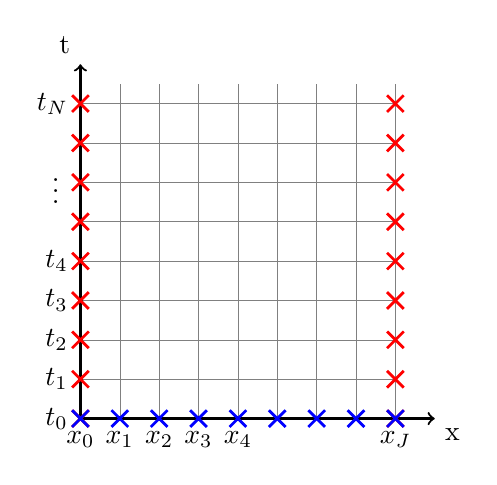
\begin{tikzpicture}[domain=0:4]
	%Grid
	\draw[step=5mm,very thin,color=gray] (0,0) grid (4,4.25);
	%Axis
	\draw[thick,->] (0,0) -- (4.5,0) node[below right] {x};
	\draw[thick,->] (0,0) -- (0,4.5) node[above left] {t};
	\foreach \x in {0,1,2,3,4}
	\draw (5*\x mm,1pt) -- (5*\x mm,-1pt) node[below] {$x_\x$};
	\node[below] at (3,-4pt){$\hdots$};
	\node[below] at (4,-1pt){$x_J$};
	\foreach \y in {0,1,2,3,4}
	\draw (1pt,5*\y mm) -- (-1pt,5*\y mm) node[left] {$t_\y$};
	\node[left] at (-4pt,3){$\vdots$};
	\node[left] at (-1pt,4){$t_N$};
	%Data
	\foreach \x in {0,...,8}{
		\draw[rotate around={45:(0,5*\x mm)},red, line width=1pt] (0.15,5*\x mm) -- (-0.15,5*\x mm);
		\draw[rotate around={135:(0,5*\x mm)},red, line width=1pt] (0.15,5*\x mm) -- (-0.15,5*\x mm);
	}
	\foreach \x in {0,...,8}{
		\draw[rotate around={45:(4,5*\x mm)},red, line width=1pt] (4.15,5*\x mm) -- (3.85,5*\x mm);
		\draw[rotate around={135:(4,5*\x mm)},red, line width=1pt] (4.15,5*\x mm) -- (3.85,5*\x mm);
	}
	\foreach \y in {0,...,8}{
		\draw[rotate around={45:(5*\y mm,0)},blue, line width=1pt] (5*\y mm,0.15) -- (5*\y mm,-0.15);
		\draw[rotate around={135:(5*\y mm,0)},blue, line width=1pt] (5*\y mm,0.15) -- (5*\y mm,-0.15);
	}
	\end{tikzpicture}
	\caption{Datos iniciales y de contorno}
	\label{fig:calor_1}
\end{figure}

Gráficamente, los datos que tenemos se pueden ver en la figura \ref{fig:calor_1}. En color rojo se muestran los datos de contorno, que en este caso son todos $0$ puesto que tenemos $u(0,t) = u(1,t) = 0$. En color azul se muestran los datos iniciales, que corresponden con los valores de la función proporcionada $u_0(x)$. En la figura también se puede ver cómo se ha realizado un mallado del espacio para aplicar el método.

A partir de estos datos se construye el algoritmo vectorial de la siguiente forma:
\begin{equation*}
	\begin{array}{l l l}
		\begin{bmatrix}
			U_1^{n+1}\\
			U_2^{n+1}\\
			\vdots\\
			U_{j-1}^{n+1}\\
		\end{bmatrix}
		=
		\begin{bmatrix}
			1-2\nu & \nu       &        & \\
			\nu    & \ddots    & \ddots & \\
			          & \ddots & \ddots & \nu\\
			          &        & \nu    & 1-2\nu\\
		\end{bmatrix}
		\begin{bmatrix}
			U_1^{n}\\
			U_2^{n}\\
			\vdots\\
			U_{j-1}^{n}\\
		\end{bmatrix}
	\end{array}
\end{equation*}

Gráficamente, lo que estamos realizando es obtener una aproximación (utilizando la aproximación de las derivadas) del siguiente punto de la partición en la derivada temporal a partir del punto anterior, el actual y el siguiente en la derivada espacial (ver figura \ref{fig:calor_2}). De esta forma, sólo usando los datos iniciales y de contorno obtenemos un valor para cada uno de los puntos del mallado.

\begin{figure}[h]
	\centering
	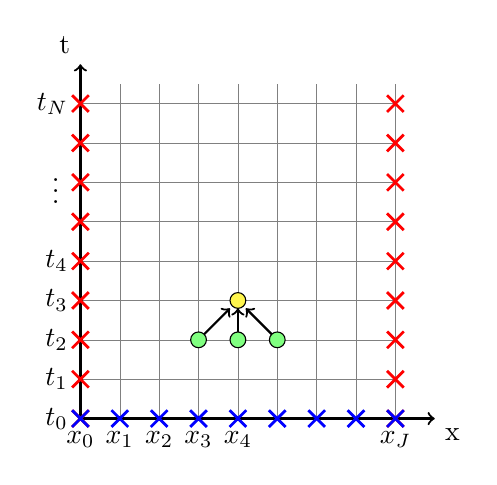
\begin{tikzpicture}[domain=0:4]
	%Grid
	\draw[step=5mm,very thin,color=gray] (0,0) grid (4,4.25);
	%Axis
	\draw[thick,->] (0,0) -- (4.5,0) node[below right] {x};
	\draw[thick,->] (0,0) -- (0,4.5) node[above left] {t};
	\foreach \x in {0,1,2,3,4}
	\draw (5*\x mm,1pt) -- (5*\x mm,-1pt) node[below] {$x_\x$};
	\node[below] at (3,-4pt){$\hdots$};
	\node[below] at (4,-1pt){$x_J$};
	\foreach \y in {0,1,2,3,4}
	\draw (1pt,5*\y mm) -- (-1pt,5*\y mm) node[left] {$t_\y$};
	\node[left] at (-4pt,3){$\vdots$};
	\node[left] at (-1pt,4){$t_N$};
	%Data
	\foreach \x in {0,...,8}{
		\draw[rotate around={45:(0,5*\x mm)},red, line width=1pt] (0.15,5*\x mm) -- (-0.15,5*\x mm);
		\draw[rotate around={135:(0,5*\x mm)},red, line width=1pt] (0.15,5*\x mm) -- (-0.15,5*\x mm);
	}
	\foreach \x in {0,...,8}{
		\draw[rotate around={45:(4,5*\x mm)},red, line width=1pt] (4.15,5*\x mm) -- (3.85,5*\x mm);
		\draw[rotate around={135:(4,5*\x mm)},red, line width=1pt] (4.15,5*\x mm) -- (3.85,5*\x mm);
	}
	\foreach \y in {0,...,8}{
		\draw[rotate around={45:(5*\y mm,0)},blue, line width=1pt] (5*\y mm,0.15) -- (5*\y mm,-0.15);
		\draw[rotate around={135:(5*\y mm,0)},blue, line width=1pt] (5*\y mm,0.15) -- (5*\y mm,-0.15);
	}
		\draw[thick,->] (1.5,1) -- (1.9,1.4);
		\draw[thick,->] (2,1) -- (2,1.4);
		\draw[thick,->] (2.5,1) -- (2.1,1.4);
	\draw[fill=green!50!white, draw=black] (1.5,1) circle (1mm);
	\draw[fill=green!50!white, draw=black] (2,1) circle (1mm);
	\draw[fill=green!50!white, draw=black] (2.5,1) circle (1mm);
	\draw[fill=yellow!70!white, draw=black] (2,1.5) circle (1mm);
	\end{tikzpicture}
	\caption{Método en diferencias finitas: $U_j^{n+1} = U_j^n+\nu\left(U_{j+1}^n - 2 U_j^n + U_{j-1}^n\right)$}
	\label{fig:calor_2}
\end{figure}
\section{Lógica de primer orden (o de predicados)}
\subsection{Exposición informal y ejemplos}
Asumimos que todos los conjuntos usados para definir el lenguaje son disjuntos. Usaremos:
\begin{itemize}
	\item \textbf{Símbolos} lógicos y de puntuación:
	$$\{\neg, \vee, ),(, ``," \}$$
	También usaremos los demás símbolos logicos como abreviaciones.
	\item Tendremos un conjunto infinito numerable de \textbf{variables}:
	$$Var = \{v_1, v_2, \hdots\}$$
	Aunque en la práctica usaremos $x,y,z$.
	\item Un conjunto de constantes, que podría ser vacío:
	$$Con = \{C_0, C_1, \hdots\}$$
	\item Funciones:
	$$Fun = \{f_0, f_1, \hdots\}$$
	\item Relaciones o predicados:
	$$Rel = \{R_1, R_2, \hdots\}$$
	\item Cuantificadores:
	$$\{\forall, \exists\}$$
	Podemos considerar $\exists x(P(x))$ como abreviación de $\neg (\forall x(\neg P(x)))$.
\end{itemize} 

No se puede cuantificar sobre constantes, funciones y relaciones en lógica de primer orden. En segundo orden, se permite cuantificar sobre funciones y predicados.

\begin{example}[Expresiones de primer orden] 

Sabemos que $P(x) \implies P(x)$, donde $x$ es libre, es cierto. Por otro lado $\forall x(P(x)\implies P(x))$ tiene el mismo significado, pero $x$ ahora es una variable ligada al cuantificador.
\end{example}

\begin{example}[Expresion de segundo orden] 

La expresión 
\[\forall P \forall x (P(x)\implies P(x))\]
es una expresión de segundo orden al estar cuantificando sobre predicados.
\end{example}

\begin{mdframed}
	\textbf{Principio de inducción matemática en $\mathbb{N}$}:
	$$\forall P (\left[P(0)\y (\forall n(P(n)\implies P(n+1)))\right]\implies \forall n(P(n)))$$
	Es una fórmula de segundo orden.
\end{mdframed}
En una lógica de primer orden, en vez de ``principio'', tenemos un ``esquema de principios'': Un principio de inducción por cada $P$.

\begin{example}[Axiomas de la teoría de grupos: Lenguaje $L_G$]\mbox{}

\begin{itemize}

	\item Axiomas:
	\begin{itemize}
		\vspace{-3mm}
		\item $\varphi_1: \forall x\forall y\forall z ((x\cdot y)\cdot z) = (x\cdot(y\cdot z))$
		\item $\varphi_2: \forall x(x\cdot e = e\cdot x = x)$
		\item $\varphi_3: \forall x\exists y (x\cdot y = e)$
	\end{itemize}

	\item Funciones:
	$$Fun = \{\cdot\}$$
	
	\item Relaciones:
	$$Rel = \{=\}$$
	
	\item Constantes:
	$$Con = \{e\}$$
\end{itemize}

Un grupo es cualquier modelo de $T_G = \{\varphi_1, \varphi_2, \varphi_3\}$. 

Veamos ahora si podemos demostrar, a partir de $T_G$ la proposición 
\[\psi: \forall x\forall y(x\cdot y = y\cdot x)\]

Es decir, queremos ver si $T_G\vdash \psi$. 

En esta ocasión es algo sencillo ver que si $G$ es no abeliano, entonces $G\nvDash \psi$, como conclusión tenemos $T_G\nvdash \psi$. Es decir, un $G$ no abeliano sería un modelo de $T_G$, puesto que satisface $\varphi_1, \varphi_2$ y $\varphi_3$ pero no es conmutativo y por tanto no satisface $\varphi_4$. 

Esto es un ejemplo de que el teorema de validez también es cierto en lógica de primer orden.
$$T_G\vdash \psi \implies T_G \vDash \psi$$

Equivalentemente
$$T_G\nvDash \psi \implies T_G \nvdash \psi$$

¿Podemos probar entonces que $T_G\vdash \neg \psi$? No, porque si tomamos un conjunto $G_2$ abeliano, entonces $G_2\nvDash \neg\psi$ y por tanto, por validez, $T_G\nvdash \neg \psi$.

Como conclusión, tenemos que $T_G$ no es una teoría completa.
\end{example}

\begin{defn}[Clausura universal]
	La clausura universal de $\phi$ es $\forall x_1, \forall x_2,\hdots, \forall x_n \phi$, donde $x_1, x_2, \hdots, x_n$ son todas las variables que aparecen libres en $\phi$.
	
	\textbf{Abreviación}: $\forall x\in z$ $(\phi(x))$ es abreviación de $\forall x ((x\in z) \y \phi (x))$.
	
	\textbf{Abreviación}: $\exists ! x(\phi (x))$ abrevia $\exists x(\phi (x) \y (\forall \phi(y) (\phi \implies y = x)))$.
\end{defn}

\begin{example}
	La clausura universal de $x < 5 + y$ es $$\forall x\forall y (x < 5 + y)$$ que tiene valor de verdad \textbf{falso}.
\end{example}

\subsection{Axiomas de ZFC (Zermelo-Fraenkel con Elección)}
	Todos son conjuntos, hereditarios y bien fundados.
	No hay ``urelementos''\footnote{Se utiliza el prefijo alemán ``ur'' que significa primordial} o átomos.
	\begin{enumerate}
		\item \textbf{Axioma del conjunto vacío} Existe un conjunto vacío, representado por $\emptyset$. Formalmente:
		$$\exists z (\forall x (x\notin z))$$
		(En el lenguaje de la teoría de conjuntos $L_S$, tenemos las relaciones binarias $\{\in, =\}$. Por otro lado $Fun: \emptyset$, $Cons: \emptyset$).

		\item \textbf{Axioma de extensionalidad}.
		Dos conjuntos son iguales únicamente si contienen los mismo elementos. Formalmente:
		$$\forall x\forall y(\forall z (z\in x\iff z\in y)\iff x = y)$$
		\begin{corol}
			El conjunto vacío es único.
		\end{corol}
		
		\item \textbf{Esquema axiomático de especificación\footnote{También conocido como esquema de axiomas de compresión}}. Sea $\phi(u)$ una fórmula de un lenguaje de primer orden que contenga una variable libre $v$. Entonces, para cualquier conjunto $x$ existe un conjunto $y$ cuyos elementos son aquellos elementos de $a$ y $x$ que cumplen $\phi(a)$. Formalmente:

		\[\forall z \exists y \forall x(x\in y\iff((x\in z)\y \phi))\]

		Las FBF permiten definir subconjuntos y hablar de subconjuntos permite evitar \concept{la paradoja de Russel}:
		
		Tenemos un axioma por cada $\phi\in FBF(L_S)$, que se define formalmente como:
		$$\forall z \exists y \forall x(x\in y\iff((x\in z)\y \phi(x)))$$
		
		Si no tuvieramos $z$, el ``axioma'' quedaría así.
		
		$$\exists y \forall x (x\in y\iff \phi(x))$$
		
		Si tomamos $\phi: x\notin x \;\; (\equiv\neg (x\in x))$
		$$\exists y \forall x (x\in y\iff x\notin x)$$
		Sabemos que $\exists y$, digamos $y_0$.
		$$\forall x (x\in y_0 \iff x\notin x)$$ 
		Como tenemos el cuantificador $\forall x$, podemos sustituir $x$ por $y_0$, obteniendo
		$$y_0\in y_0 \iff y_0\notin y_0$$
		Que es una contradicción. 

		Para evitar llegar a esta contradicción añadimos $z$ como se ha hecho.
		
		\begin{obs}

			$\{z_1,\hdots, z_n\}$ es un conjunto.
			
			$S(n) = \{0, \hdots, n\}$ es un conjunto.
			
			$y=\{1, \hdots, n\} = \{x\in S(n)\tq x>0\}$ es un conjunto.
			
			La función $f(i) = z_i$ es una función (conjunto de pares ordenados). Por el axioma de reemplazo, el rango $f$ es un conjunto. Donde $f:\{1,\hdots, n\}\to \{z_1, \hdots, z_n\}$.
		\end{obs}
		
		\item \textbf{Axioma de emparejamiento.} Si $x$ e $y$ son conjuntos, el par $\{x, y\}$ es un conjunto. Si $z$ es un conjunto, $\{\{x,y\},z\}$ es un conjunto. Si $x = y$, entonces obtenemos $\{x,x\} = \{x\}$. Formalmente
		$$\forall x\forall y\exists z\forall u(u\in z\iff \left[(u=x)\Or (u=y)\right])$$
		$z$ es $\{x,y\}$, si $x=y$, $z$ es $\{x,x\}=\{x\}$.
	\end{enumerate}
	
	Antes de seguir enunciado los axiomas veamos algunas definiciones de términos ya conocidos vistos desde otro enfoque:
	
	\begin{defn}[Los naturales]
	\begin{itemize}
		\item $0:=\emptyset$
		\item $1:=\{\emptyset\}$ (por emparejamiento o partes cuando lo veamos).
		\item $2:=\{\emptyset, \{\emptyset\}\} = \{0,1\}$ (por emparejamiento).
		\item $3:=\{1,2,3\} = \{\emptyset,\{\emptyset\},\{\emptyset, \{\emptyset\}\}\}$ (Por el axioma 4).
	\end{itemize}
	\end{defn}

	\begin{defn}[Sucesor]
		El sucesor de $n$, $S(n)$ es $$S(n) = \{0,1,2,\hdots, n\}$$
	\end{defn}
	
	\begin{defn}[Suma en los naturales]
		$n+1 := S(n)$. Si hemos definido $n+m$, entonces
		$n+m+1 := S(n+m)$.
	\end{defn}

	\obs A partir de aquí podemos definir todo $n\in \nat$ como un conjunto, pues $n=S(n-1)=\{0,1,...,n-1\}$
	
	\begin{defn}[Producto de los naturales]
		En cuanto al producto:
		\begin{itemize}
			\item $n\cdot0 = 0$
			\item $n\cdot1=n$
			\item Si $n\cdot m$ está definido, entonces $n(m+1) = n\cdot (m+1) = n\cdot m + n$.
		\end{itemize}
	\end{defn}
	
	\begin{defn}[Menor]
		$$n<m\iff n\in m$$
	\end{defn}
	
	Usando los axiomas vistos, tenemos que cada n es un conjunto, pero nada nos dice que $\mathbb{N} :=w$ sea un conjunto, o que exista un conjunto infinito.

	Prosigamos viendo \textbf{axiomas de ZFE}
	
	\begin{enumerate}
	\setcounter{enumi}{4}
		\item \textbf{Axioma de la unión.} Dada cualquier colección de conjuntos $\algb{C}$, existe un conjunto representado por $\bigcup \algb{C}$ llamado \textit{unión de }$\algb{C}$, que contiene todos los elementos de cada conjunto $\algb{C}$. Esto es:
		 
		 $$\forall x \exists y \forall z (z\in y\iff\exists u((u\in x)\y (z\in u)))$$
		 
		 Se usa al definir $$S(n) = \{0, 1,\hdots,n\} = n\cup \{n\}$$
		 
		 Nos permite definir cada $n$ como un conjunto, pero nada nos dice que $\mathbb{N}$ sea un conjunto.		 
		 \begin{example}
			Sea $X=\{1,\{2\},\{2,3\}\}$, entonces
			$$\cup X = \{0, 2, 3\}$$ porque $1=\{\emptyset\}$.
		 \end{example}
		 
		 \item \textbf{Esquema axiomático de reemplazo}. Si $\phi(a,b)$ es una sentencia tal que para cualquier elemento $a$ de un conjunto $x$ el conjunto $y=\{b | \phi(a,b)\}$ existe, entonces existe una función $\appl{f}{x}{y}$ tal que $f(z)=y$. Formalmente

		 $$\forall a \left[\forall x\in a ((\exists! y (\varphi(x,y))))\implies (\exists z \forall x \in a \exists y \in z (\varphi(x,y)))\right]$$
		 
		 Este axioma nos dice que para definir una función, $Ran f$ debe pertenecer a un conjunto preexistente. En particular, $Ranf$ no es ``cofinal'' en el universo de los conjuntos.
		 
		 \item \textbf{Axioma de fundación.\footnote{También conocido como axioma de regularidad}}. Para todo conjunto no vacío $x$ esite un subconjunto $y \in x$ tal que $x \cap y = \emptyset$

		 $$\forall x \left[(x\neq \emptyset)\implies (\exists y \in x (\forall z \in x (z\notin y)))\right]$$
		 
		 Este axioma implica que para todo conjunto $z$, $z\notin z$. Supongamos que existe un $z$ tal que $z\in z$. Entonces, aplicamos el axioma de fundación al conjunto $\{z\}$, porque $z$ no es vacío (al contener a $z$).  $\{z\}$ es un conjunto por pares y extensión, $\{z,z\} = \{z\}$ o por compresión: $\{y : y\in z \y  y=z\}$.
		 
		 Por el axioma, $\exists y\in\{z\}$ tal que $z\cap y=\emptyset$. Pero $y=z$ luego $z\cap y = z \neq \emptyset$. Luego para todo conjunto, $z\notin z$.
		 
		 \begin{obs}
		 	Si hubiese un $z\in z$, entonces $z\ni z\ni z\ni z\hdots$. Obtendríamos una cadena infinita descendiente de $\in$.
		 	Pude demostrarse que este axioma prohibe todas las cadenas infinitas descendientes y los bucles tales como $z_1\ni z_2\ni \hdots \ni z_n \ni z_1$.
		 \end{obs}
		 
		 \item \textbf{Axioma del conjunto potencia\footnote{También conocido como axioma de partes}}. Para cualquier conjunto $x$ existe otro conjunto, representado por $\algb{P}(x)$, que contiene a todos los subconjuntos de $x$. Formalmente.

		 \[\forall x \exists y \forall z (z \in y \iff \forall a (a\in z \implies a \in x))\]
		 
		 \textbf{Par ordenado:} si $x$ e $y$ son conjuntos $(x,y):=\{x, \{x,y\} \}$ podemos definir funciones, relaciones, etc. Hemos construido cada $n$ con $n$ elementos. Sea $X$ un conjunto ya construido (por tanto, finito)
		 $$X,Y \subset \mathbb{N}, f:X\to Y$$
		 
		 $Ran f \subset N = \{0, \hdots, N-1\}$ conjunto ya construido. Podemos tomar $N = \max \{f(x): x \in X\} + 1$.
		 
		 En general $Card(\mathcal{P}(X)) = 2^{Card(X)}$.
		 
		 \textbf{Abreviación: } Usamos $z\subset X \equiv \forall w((w\in z)\implies (w\in X))$
		 $\forall X \exists y \forall z(z\subset X\iff x\in y)$.
		 
		 \textbf{Nota aleatoria:}
		 
		 $\mathbb{R}^1 = \mathbb{R}^{\{\emptyset\}} = \{(\emptyset, x): x\in\mathbb{R}\}$
		 
		 $\mathbb{R}^2 = \mathbb{R}^{\{0,1\}} = \{f:(0,1)\to \mathbb{R}\} = \{(x_0, x_1): x_0, x_1 \in \mathbb{R}\}$
		 
		 $\mathbb{R}^0 = R^\emptyset = \{f:\emptyset\to \mathbb{R}\}$ (es elegir 0 elementos de $\mathbb{R}$, que es lo mismo que rechazarlos todos, lo cual sólo hay una forma de hacerlo, que es nuestra constante).
		 
		 \item \textbf{Axioma de infinitud.} Existe un conjunto $x$ tal que $\emptyset \in x$ y tal que si $y\in x$, entonces $y \cup \{y\}\in x$. En símbolos:

		 $$\exists x ((\emptyset\in x)\y (\forall y(y\in x \implies y\cup \{y\} \in x)))$$
		 
		 A partir de este conjunto, definimos $\mathbb{N} = \omega$ exigiendo que todo elemento distinto del 0 sea sucesor de otro elemento. Sea $X$ un conjunto dado por el axioma de infinitud.
		 $$\mathbb{N}:= \{x\in X:\left[\exists y \in X (x=y\cup \{y\})\y (\forall w\in x (w=0\Or (\exists z(w=z\cup \{z\}1)))) \right]\}$$
		 
		 \textbf{Ejemplo informal:}
		 
		 $\mathbb{N}_0:=\{(0, n): n\in \mathbb{N}\}\equiv \mathbb{N}$
		 
		 $\mathbb{N}_1:=\{(1, n): n\in \mathbb{N}\}\equiv \mathbb{N}$
		 
		 Luego $\mathbb{N}_0\cup\mathbb{N}_1$ con el orden del diccionario es $\{(0,0), (0,1), (0,2), \hdots, (1,0),(1,1), (1,2), \hdots\}$
		 
		 Por inducción: Sea $S\subset\mathbb{N}$. Si $0\in S\y(\forall n(n\in S\implies n+1\in S))$. En conclusión, $\mathbb{N}\subset S. (S\subset \mathbb{N}\implies \mathbb{N}=S)$
		 
		 \item \textbf{Axioma de elección.} Dada una familia de conjuntos no vacíos podemos coger un elemento de cada conjunto. Este axioma puede expresarse de manera equivalente a, dado un conjunto cualquiera $x$, existe una función f que elige un elemento de cada conjunto no vacío de $x$. Formalmente
		 
		 $$\forall X(\emptyset\notin X \implies \left[ \exists f:X\to\cup X (\forall t\in x(f(t)\in t))\right])$$
		 		 
		 Hay que notar que al cuantificar funciones estamos pasando a lógica de segundo orden.
		 
		 Si $\mathcal{C}=\{A_\alpha: \alpha\in \Lambda\}$ es una colección de conjuntos disjuntos no vacíos, $\exists f:\mathcal{C}\to \cup\mathcal{C}$ tal que $$\forall A_\alpha \in \mathcal{C}, f(A_\alpha)\in A_\alpha$$
		 
		 Luego escrito en primer orden:
		 
		 $\forall y\forall u (u\subset P(y) \y \forall z\forall w\left[(z\in u \y w\in u)\implies (z\neq \emptyset\y (z = w \Or z\cap w = \emptyset ))\right]\implies \exists x \in P(y) (\forall z \in u \exists v (x\cap z = \{v\})))$
		 		 
		 El axioma de elección es equivalente al lema de Zorn, que es equivalente a que todo conjunto tiene un buen orden.
		 
		 Algunas consecuencias:
		 \begin{itemize}
		 	\item Todo conjunto infinito contiene un conjunto numerable.
		 	\item Toda relacion contiene a una función con el mismo dominio.
		 	\item Todo espacio vectorial tiene una base.
		 	\item Existen conjuntos en $[0,1]$ que no son medibles con respecto a la medida de Lebesgue.
		 	\item Si \textbf{AP} (axiomas de Peano) es completa, puede extenderse a una teoría completa.
		 \end{itemize}
	\end{enumerate}
	
\subsection{Axiomas de Peano}
	Los 5 Axiomas de Peano son:
	\begin{enumerate}
		\item Existe un número natural 1. En otros términos,1 está en N, el conjunto de los números naturales.
		\item Todo número natural n tiene un sucesor n* (este axioma es usado para definir posteriormente la suma).
		\item 1 no es el sucesor de algún número natural.
		\item Si hay dos números naturales n y m con el mismo sucesor, entonces n y m son el mismo número natural.
		\item Si 1 pertenece a un conjunto K de números naturales, y dado un elemento cualquiera n, el sucesor n* también pertenece al conjunto K, entonces el conjunto K debe ser el conjunto de todos los números naturales. Este axioma es el principio de inducción matemática.
	\end{enumerate}

	\begin{theorem}
		$\mathbb{N}$ es único en el sentido de que si $A$ y $B$ satisfacen los axiomas de Peano, entonces $A=B=\mathbb{N}$. 
	\end{theorem}
	\begin{proof}
		Por hipótesis, $0\in A\cap B$.

		Si $n\in A\cap B$ entonces $n+1\in A\cap B$. Por lo tanto $A=B=A\cap B=\mathbb{N}$.
	\end{proof}
	
	Hasta ahora hemos visto que
	\begin{itemize}
		\item Los axiomas de la teoría de grupos: admiten muchos modelos muy distintos.
		\item Axioma de Peano: intentan caracterizar a $\mathbb{N}$. Hay varios conjuntos que satisfacen los axiomas de Peano, estos modelos son todos isomorfos.
	\end{itemize}

La gran ventaja que nos aporta la lógica de primer orden es que permite expresar los axiomas de ZFC que fundamentan la mayor parte de las matemáticas (en particular ZF $\Rightarrow$ Axiomas de Peano (1 orden))

\subsection{Introducción a lógicas de segundo orden}

En la práctica, usamos constantemente lógicas de segundo orden sin preocuparnos de si los conjuntos son demasiado grandes
\begin{example}
\textbf{Teorema:} Sea K un espacio topológico compacto y sea $f: K \rightarrow \mathbb{R}$ continua. Entonces f alcanza sus valores máximo y mínimo.

\textbf{Traducción semiformal:} Sea $\algb{C}$= clase de todos los conjuntos compactos, y sea:
$$F_k = \{f: K \rightarrow \mathbb{R} | \text{f es continua}\}$$

Entonces nos queda:
$$\forall K \in \algb{C} \textbf{ }\forall f \in F_k \left( \exists a,b,c \in K \left( \forall x \in K \left( f(a) \leq f(x) \leq f(b) \right) \right) \right)$$

\textbf{OJO:} $\algb{C}$ es el conjunto de todos los conjuntos.

De modo que, una manera de interpretar el teorema anterior en una lógica de primer orden es considerar que tenemos un esquema de teoremas, es decir, tenemos un teorema por cada $(K,f)$ donde $K$ y $f$ pueden describirse en el lenguaje.
\end{example}


No usamos la lógica de 2º orden todo el tiempo porque compacidad, y por tanto completitud, fallan.

\begin{theorem}
Existe una teoría T en un lenguaje de 2º orden, tal que, todo subconjunto finito de T tiene un modelo, pero T no tiene ningún modelo.
\end{theorem}
\begin{proof}
Si consideramos la teoría $\Psi_{\infty}$, donde $\Psi_{\infty}$ nos dice que existe una función inyectiva que no es sobreyectiva, vemos que todos sus modelos son infinitos (todas las funciones que satisfacen la teoría deben moverse entre conjuntos infinitos.)
$$ \Psi_{\infty}: \exists f \left(\forall x \textbf{ } \forall y \left( \left( f(x)=f(y)\right) \Rightarrow x=y \right) \y \left( \exists z \forall x \left( z \neq f(x) \right) \right) \right) $$


Por otro lado, es claro que todo modelo de $\neg \Psi_{\infty}$ es finito.

Vamos a considerar el conjunto de teorías $\Psi_n$, cada una de las cuales nos dice que por lo menos hay n objetos distintos:
$$ \Psi_2: \exists v_1 \exists v_2 \left(v_1 \neq v_2 \right) $$
$$ \Psi_3: \exists v_1, v_2, v_3 \left( \left(v_1 \neq v_2 \right) \y \left(v_2 \neq v_3 \right) \y \left(v_1 \neq v_3 \right) \right) $$
$$\vdots$$
$$ \Psi_n: \exists v_1,..., v_n \left( \y _{1\leq i < j \leq n} \left(v_i \neq v_j \right)  \right) $$

Consideramos ahora la teoría formada por la unión de estas teorías.
$$T = \left\{ \neg \Psi_{\infty}, \Psi_n : n \in \mathbb{N} \setminus \left\{0,1\right\} \right\}$$

Sea $\epsilon \subset T$ un subconjunto finito, si $\epsilon = \{\neg \Psi_{\infty} \}$, $1=\{0\}$ es un modelo.

Si para algún n, $\Psi_n \in \epsilon$, llamamos N al natural más grande tal que $\Psi_n \in \epsilon$. Entonces $N=\{0,1,...,N-1\}$ es un modelo de $\epsilon \cup \{\neg \Psi_{\infty} \}$ y, por tanto, un modelo de $\epsilon$.

Pero T no tiene modelos, porque cualquier modelo debe ser a la vez finito (por $\neg \Psi_{\infty}$) y contener al menos n elementos distintos $\forall n \in \mathbb{N}$, con lo que llegamos a una contradicción.
\end{proof}


\subsection{Completitud}

\begin{theorem}[Teorema de completitud]
Sea T una teoría en el lenguaje de primer orden, existen dos versiones de este teorema.
\begin{enumerate}
\item $T \vdash \phi \Leftrightarrow T \vDash \phi$

\item $T \text{ es consistente } \Leftrightarrow T \text{ tiene un modelo }$
\end{enumerate}
\end{theorem}

\begin{proof}
\begin{enumerate}
\item 
Ya hemos visto como demostrar ambos sentidos de la implicación

$\Rightarrow)$ Por validez.\\
$\Leftarrow)$ Por Gödel (Henkin)

\item
\end{enumerate}
\end{proof}

\textbf{Corolario:} Compacidad: Sea T una teoría en un lenguaje de primer orden. T tiene un modelo $\Leftrightarrow$ todo subconjunto finito de T tiene un modelo.

En todos los lenguajes de primer orden \textbf{siempre} tenemos símbolos lógicos, incluyendo, o no, igualdad, signos de puntuación (paréntesis y comas), cuantificador(es) y variables, de modo que estos signos no se incluyen al describir un lenguaje.

\begin{example}
\textbf{Lenguaje de la aritmética}
\[L_{Arit} = \{\underbrace{0,1}_{\text{constantes}},\underbrace{+,\cdot}_{\text{funciones binarias}}, \underbrace{<}_{\text{relaciones binarias}}\}\]
\end{example}

\begin{theorem}[Primer teorema de incompletitud de Gödel]
Sea $T$ una teoría en (un lenguaje de primer orden) \textbf{axiomatizable}\footnote{Tenemos un procedimiento para comprobar si cada FBF es un axioma o no}. Si el lenguaje contiene, al menos, el lenguaje de la aritmética y la teoría contiene a los \textbf{axiomas de Peano} entonces 
\[T \text{ consistente } \implies T \text{ incompleta}\]
\end{theorem}

\begin{theorem}[Teorema de Presburger y Skolem]
Each sentence in the languaje of the structure $(\ent;0,1,+,-,<)$ that is true in this structure is provable from the axioms for ordered abelian groups with least positive element 1, augmented, for each $n=2,3,4,...$ by an axiom that says that for every $a$ ther is a $b$ such that $a=nb$ or $a=nb+1$ or ... or $a+nb+1+...+1$ (with $n$ disjuncts in total).

Moreover, there is an algorithm that, given any sentence in this languaje as input, decides whether this sentence is true in $(\ent; 1,0,+,-,<)$.
\end{theorem}


\begin{theorem}[Segundo teorema de incompletitud de Gödel]
Sea $T$ una teoría en un lenguaje de primer orden \textbf{axiomatizable} y consistente, si $T$ tiene, al menos, el poder expresivo de la aritmética de Peano, es posible escribir una sentencia que llamaremos $CON(T)$, que puede interpretarse como ``T es consistente'' y que \textbf{no puede ser probada}, es decir, $T \nvdash CON(T)$
\end{theorem}

\begin{obs}
Si $T$ es consistente entonces $T \nvdash \neg CON(T)$.

$CON(T)$ puede interpretarse como ``T es consistente", luego existe un modelo $a$ de $T$ con $a \vDash CON(T)$ y, por tanto, $a \nvDash \neg CON(T)$.

En consecuencia, si $T$ es consistente, entonces $T \cup \{ CON(T)\}$ y $T\cup \{\neg CON(T)\}$ son extensiones consistentes de $T$, luego ambas teorías tienen modelos.

\end{obs}

\begin{obs}
Los axiomas de Peano son teoremas en ZF luego los resultados anteriores se aplican a ZF.
\end{obs}

\begin{theorem}
Si ZF es consistente, entonces $ZF \nvdash CON(ZF)$
\end{theorem}

\begin{theorem}[Teorema de Cantor] 
Cantor probó que 
\[card(\nat) < card(\real)\]
por diagonalización.

Además, Cantor conjeturó que \textbf{no existe} ningún conjunto $E$ tal que
\[card(\nat) < card(E) < card(\real)\]
A esta conjetura se la denomina la \textbf{hipótesis del continuo (CH)}
\end{theorem}

Aunque Cantor invirtió mucho tiempo tratando de demostrar su conjetura, no fue capaz de conseguir nada. Esta falta de éxito se debió a que los axiomas ZF no son suficientemente fuertes como para demostrar la conjetura.

\begin{theorem}
Si ZF es consistente, entonces también lo son:
\begin{enumerate}
\item ZF + C + CH (Gödel finales años 30)
\item ZF + $\neg$C + CH (Paul Cohen finales años 60)
\item ZF + C + $\neg$CH (Paul Cohen finales años 60)
\item ZF $\neg$C + $\neg$CH (Paul Cohen finales años 60)
\end{enumerate}

Donde $C$ representa el axioma de elección.
\end{theorem}

\textbf{Llegados a este punto es recomendable para el lector la lectura del apartado 2.3 del libro}

\subsection{Lenguajes y estructuras}

\begin{defn}[Lenguaje de primer orden]
$L$ es un \textbf{lenguaje de primer orden} si es unión disjunto de los siguiente conjuntos:
\begin{enumerate}
\item Símbolos lógicos y de puntuación
\[\{\neg, \to , = , ), (, ``,''\}\]
\item Variables, que quedan representadas por el conjunto infinito numerable
\[Var = \{v_0,v_1,...\}\]
\item Constantes (podría ser vacío)
\item Funciones (podría ser vacío)
\item Relaciones o predicados (podría ser vacío)
\item Cuantificador $\{\forall \}$ considerando el cuantificador $\exists$ como negación del $\forall$.
\end{enumerate}
\end{defn}

Una L-estructura es una interpretación del lenguaje $L$, y si $T$ es una teoría en $L$ entonces un modelo de $T$ es una L-estructura donde todas las fórmulas en $T$ son verdad.

Esta afirmación establece una relación entre diferentes términos que aún no hemos definido. Vamos a verlos:

\begin{defn}[L-estructura]
Una \textbf{L-estructura} $a$ es una 4-upla $a=(A,C^a,F^a,R^a)$ donde 
\begin{itemize}
\item $A\neq \emptyset$ es el conjunto al que pertenecen las variables y al que se aplican los cuantificadores
\item Por cada $c \in $ Constantes de L existe $c^a\in C^a$ asociada a $c$
\item Por cada $f \text{ n-aria } \in $ Funciones de L existe $f^a\text{ n-aria }\in F^a$ asociada a $f$
\item Por cada $r \text{ n-aria }\in $ Relaciones de L existe $r^a \text{ n-aria }\in R^a$ asociada a $r$
\end{itemize}
Los términos denotan ``objetos'' en la interpretación, son equivalentes a ``nombres''. Así las variables serían ``nombres comunes'' y las constantes ``nombres propios''
\end{defn}

\begin{defn}[Término]
Los \textbf{términos} son la clase de fórmulas más pequeña que se obtiene mediante aplicación de la siguiente regla
\begin{enumerate}
\item Las variables son términos
\item Las constantes son términos
\item Si $t_1...t_n$ son términos y $f$ es una función n-aria entonces $f(t_1,...t_n)$ es un término.
\end{enumerate}
\end{defn}

\begin{defn}[Fórmulas atómicas]
Las \textbf{fórmulas atómicas} son 
\begin{enumerate}
\item Por cada relación n-aria $R$ y términos $t_1...t_n$, $R(t_1,...,t_n)$ es una \textbf{fórmula atómica}.
\item Si $t_1$, $t_2$ son términos entonces $t_1=t_2$ es una \textbf{fórmula atómica}.
\end{enumerate}
\end{defn}

\begin{defn}[Fórmula bien formada]
Las \textbf{fórmulas} (bien formadas) de $L$ son la clase más pequeña cerrada bajo las siguientes operaciones
\begin{enumerate}
\item Las fórmulas atómicas son fórmulas
\item Si $\Phi,\Psi$ son fórmulas también lo son $\Phi \to \Psi$ y $\neg \Phi$
\item Si $\Phi$ es una fórmula también lo es $\forall x \Phi$
\end{enumerate}
\end{defn}

\begin{defn}[Variable ligada]
Si $x$ aparece en la fórmula $\phi$ bajo el rango de un cuantificador (ya sea $\forall$ o $\exists$), decimos que $x$ es una variable \textbf{ligada}.

En caso contrario, es decir, si $x$ aparece en $\phi$ pero no está cuantificada, decimos que $x$ es \concept{libre}
\end{defn}

\begin{defn}[Fórmula cerrada]
Decimos que $\phi$ es una \textbf{fórmula cerrada o sentencia} si no tiene variables libres.
\end{defn}

\begin{example}[Reemplazo de variables]

Consideramos al fórmula:
\[\int_0^1 xy \dif x = \frac{y}{2}\]

donde la variable $x$ está ``ligada'' por el $\dif x$ e $y$ está libre.

Vamos a ver qué términos pueden reemplazar a la variable $y$.

Por lo que sabemos de matemáticas tenemos claro que podemos sustituir la $y$ por cualquier otra variable distinta de $x$ como $z,t,v...$ y también puede sustituirse por funciones como $\sin(y)$.

En general, podrá sustituirse una variable por cualquier variable o función que no dependa variables ligadas.
\end{example}

\begin{example}
Consideramos ahora la fórmula
\[\phi: \ \forall x (x=y)\]

Podemos ver que el único modelo de esta fórmula será aquel conjunto que esté formado por un único elemento.

Dicho de forma más técnica, esta fórmula es cierta en la L-estructura $a$ si y sólo si $card(A)=1$.

Obviamente, si en este mismo ejemplo sustituimos la $y$ por una $x$, obtenemos la fórmula
\[\phi: \ \forall x (x=x)\]
que es cierta para todas las interpretaciones.
\end{example}

\begin{prop}
Si $x$ aparece libre en una fórmula $\phi$, el término $t$ puede sustituir a $x$ si ninguna de las variables de $t$ se vuelve ligada al reemplazar a $x$ por $t$.
\end{prop}

En estos ejemplos hemos estado hablando de veracidad y falsedad de afirmaciones sin haber definido previamente estos conceptos. Si bien es algo totalmente intuitivo y casi trivial, es necesario tener una definición formal de estos términos. 

Queremos por tanto una definición que nos permite saber cuándo σ es verdad en $a$, es decir, cuando $a\vDash σ$. Para ello buscaremos una definición inductiva en términos de subfórmulas más cortas.

En particular queremos definir $a \vDash \forall x \phi$ en términos de $a \vDash \phi$.

Una forma de dar sentido a $a\vDash \phi$ es extender el lenguaje $L$ a  $L_A=L\cup\{\underline{a}, a \in A\}$ considerando la unión disjunta.

\begin{example}
Supongamos que tenemos $L = \{c, f, R\}$,  $a = (\nat, 0,S, \leq)$

Dada $\sigma =\forall x(cR x)$, queremos definir $a\vDash \sigma$ en términos de setencias más cortas.

Por cada $n\in \nat$, añadimos la constante $\underline{n}$ (a $L$), cuya interpretación es $n$.

Entonces $a\vDash \sigma$, puesto que $\forall \underline{n}, n\in \nat, c\le n$, que es una sentencia más corta que $\sigma$.

Luego $L_\nat$ es la unión disjunta:
$L_{\nat} = L\cup \{\underline{n}: n\in \nat\}$
\end{example}

\begin{defn}[Consecuencia lógica]
	Vamos a ver cuándo $a\vDash \sigma$ para $L-$sentencias.

	Sea $L_A = L\cup \{\underline{a}: a \in A\}$ (unión disjunta), tenemos diferentes casos:
	\begin{enumerate}
		\item \textbf{Sentencias atómicas}

		Sean $t_1,\hdots,t_n$, $L_A-$términos sin variables diremos que 
		\[a\vDash t_1=t_2 \iff t_1^a=t_2^a\]
		y, además, para toda relación o predicado $n-$ario $P$, 
		\[a\vDash P(t_1,\hdots,t_n)\iff (t_1^a,\hdots,t_n^a)\in P^a\]

		\item \textbf{$L_A$ sentencias}

		Sean $\sigma_1$ y $\sigma_2$ $L_A$-sentencias, entonces 
		\[a\vDash \neg \sigma \iff a\nvDash \sigma, \ \ a\vDash \sigma_1\rightarrow \sigma_2\iff a\nvDash\sigma_1 \text{ ó } a\vDash\sigma_2\]

		\item \textbf{Cuantificadores}

		$a\vDash \sigma = \forall x\varphi(x)\iff \forall a \in A, a\vDash \varphi(\underline{a})$
	\end{enumerate}
\end{defn}

\begin{prop}
	Sea $\varphi$ una fórmula de $L_A$, $\varphi = \varphi(x_1,\hdots,x_n)$ 
	\[a\vDash \varphi \iff a\vDash \forall x_1,\forall x_2, \hdots, \forall x_n \varphi\]
	o equivalentemente, 
	\[\forall (\underline{a_1}, \hdots, \underline{a_n})\in A^n \implies a\vDash \varphi(\underline{a_1}, \hdots, \underline{a_n})\]
\end{prop}

\subsection{Axiomas de la lógica de primer orden y reglas de deducción}

\begin{enumerate}
	\item \textbf{Axiomas proposicionales} (los del libro) o a efectos de este curso, todas las tautologías.
	\item \textbf{Axiomas de igualdad}:
	\begin{itemize}
		\item $x=x$
		\item $x=y \implies y=x$
		\item $\left[(x=y)\y(y=z)\right]\implies x=z$
		\item Para toda $P$ $n-$aria, $\left[x_1=y_1\y \hdots\y x_n=y_n \y P(x_1, \hdots, x_n)\right] \implies P(y_1, \hdots, y_n)$
		\item Para toda función $f$ $n-$aria, $(x_1=y_1\y \hdots \y x_n=y_n)\implies f(x_1, \hdots, x_n) = f(y_1, \hdots, y_n)$
	\end{itemize}
	\item \textbf{Axioma de cuantificación}.
	
	Si el término $t$ puede sustituir en $x$, entonces
	$$\forall x\varphi(x) \implies \varphi (t|x) (= \varphi(t) \text{ abreviación})$$
\end{enumerate}

\begin{theorem}
	Si $\varphi$ es un axioma y $a$ es una $L-$estructura, entonces $a\vDash \varphi$.
	Es decir, los axiomas lógicos son verdad en todas las L-estructuras (interpretaciones).
\end{theorem}
\begin{proof}
	Son verdad para las fórmulas atómicas, por inducción.
	Por ejemplo, $a\vDash x=x$. Las demás fórmulas por inducción en el número de símbolos lógicos (incluyendo cuantificadores).
\end{proof}

\subsection{Reglas de deducción}
\begin{enumerate}
	\item \textbf{Modus Ponens:} De $\varphi$ y $\varphi\implies \Psi$ obtenemos $\Psi$.
	\item Si $x$ no aparece libre en $\varphi$, de $\varphi \implies \Psi$ deducimos que $\varphi\implies \forall x \Psi$.
\end{enumerate}

\begin{obs}
	Estas reglas de deducción preservan el valor de verdad:
	\begin{enumerate}
		\item Si $a\vDash \varphi$ y $a\vDash \varphi\implies\Psi$, entonces $a\vDash \Psi$.
		\item Si $x$ no aparece libre en $\varphi$ y $a\vDash \varphi \implies \Psi$ entonces ó $a\nvDash \varphi$ ó $a\vDash \Psi$. 
		
		Si $a\nvDash \varphi$, entonces $a\vDash \varphi \implies \text{cualquier otra cosa}$. 
		
		Si $a\vDash \varphi$, entonces, $a\vDash \Psi$.
		
		Esto significa que $\forall a\in A$ (extendemos $L\cup\{\underline{a}:a\in A \}$, unión disjunta).
		
		$\Psi (\underline{a}) = \Psi (\underline{a}|x)$ es verdad en $a$. Luego es verdad que $a\vDash \forall x\varphi(x)$.
	\end{enumerate}
\end{obs}

Muchas definiciones (y resultados) son enteramente análogos a las de la lógica proposicional.

\begin{defn}[Teoría]
	$\Sigma = \{\sigma_\alpha : \sigma_\alpha \text{ es una setencia de } L, \alpha \in \Lambda\}$
\end{defn}

\begin{defn}[Prueba]
	Como antes, sólo que en vez de una regla de deducción, hay dos.
	
	\textbf{Notación: } $\Sigma \vdash \sigma$.
\end{defn}

\begin{defn}[Modelo]
	$a$ es un modelo de $\Sigma$ si 
	$$\forall \sigma \in \Sigma, a\vDash \sigma$$
\end{defn}

\begin{defn}[Consecuencia tautológica]
	$\sigma$ es una consecuencia lógica de la teoría $\Sigma$ si para todo modelo $a$ de $\Sigma$, $a\vDash \sigma$. 
\end{defn}

\begin{example}
	Si $\Sigma =\{\text{axiomas de la teoría de grupos}\}$ y $\sigma_1$ es la sentencia que expresa la conmutatividad, $\sigma_1$ no es consecuencia lógica de $\Sigma$ (hay grupos no conmutativos). 

	Si $\sigma_2$ expresa el hecho de que el inverso por la izquierda es igual que el inverso por la derecha, entonces $\sigma_2$ es consecuencia lógica de $\Sigma$.	
\end{example}

\noindent \textbf{Notación: } $\Sigma \vDash \sigma \iff \sigma $ es consecuencia lógica de $\Sigma$. ``$\vDash$'' es una noción semántica y ``$\vdash$'' es una noción sintáctica. $\Sigma \vdash \sigma$ significa que existe una demostración formal lo cual depende de los axiomas, de las reglas de deducción y de las premisas.

\begin{example}
	Vamos a probar que si $\Sigma\vDash \forall x \varphi(x)$, entonces $\Sigma \vDash \exists x\varphi(x)$ (cuestión semántica). 

	Sea $a$ cualquier modelo de $\Sigma$. 
	\[\forall x\varphi(x) \iff \forall a\in A, a\vDash \varphi(\underline{a})\] Escogemos cualquier $b\in A\neq \emptyset$. Entonces $a\vDash \varphi(\underline{b})$, luego $a\vDash \exists x \varphi(x)$.
\end{example}

Trabajando con lógica proposicional vimos que era más sencillo comprobar que una FBF era consecuencia lógica, pues bastaba con construir su tabla de verdad, que construir una demostración o prueba de la fórmula a partir de los axiomas.

Algo similar ocurre en lógica de predicados. 
\begin{example}
Demostramos que, siendo $z$ una variable que no aparece en $\phi$ se cumple:
\[\forall x \varphi(x) \vDash \forall x \varphi(z) \ \left(= \forall z \varphi(z|x)\right)\]
Sea $a\vDash \forall x \varphi(x)$, es decir
\[\forall a \in A \ \ \varphi(\underline{a})\left(= \varphi(\underline{a}|x)\right)\]
es cierto en $a$.

Por tanto, $\forall z \varphi(z)$ es verdad en $a$.
\end{example}

\begin{example}
Vamos a probar
\[\forall x \varphi(x) \vdash \forall z \varphi(z)\]
Realizaremos la demostración por pasos:
\begin{enumerate}
\item Invocamos la premisa de la demostración:
\[\forall x \varphi(x)\]

\item Invocamos ahora el axioma de cuantificación:
\[\forall x \varphi(x) \to \varphi(x)\]

\item Aplicamos Modus Ponens con lo que obtenemos:
\[\varphi(z)\]

\item Apoyándonos en el apartado a) del ejercicio 4 de la hoja 6, invocamos:
\[\varphi \vdash \forall x \varphi\]

\item Combinando los dos últimos resultados llegamos a:
\[\varphi(z) \vdash \forall z \varphi(z)\]
\end{enumerate}

\end{example}

\begin{prop}
Toda teoría consistente puede extenderse a una teoría $M$ consistente y maximal (con respecto a la inclusión). 
\end{prop}

La demostración de esta proposición se basa en el empleo del Teorema de Lendenbaum usando zorn.

\begin{prop}
La teoría $M$ consistente y maximal, mencionada en la proposición anterior, es completa
\end{prop}
\begin{proof}
Sabemos que 
\[\forall \varphi, \ \varphi \in M \Or \neg \varphi \in M\]
puesto que la teoría es maximal, si $\varphi, \neg \varphi \notin M$ podríamos añadir una de ellas a $M$ con lo que entonces $M$ no sería maximal. Por tanto no es posible esta situación.

Por tanto, siempre tendremos una de dos:
\[M \vdash \varphi \Or M \vdash \neg \varphi\]
siendo la demostración trivial y de una sola línea pues $\varphi $o $\neg \varphi$ deben pertenecer a $M$, como hemos visto en el párrafo anterior.
\end{proof}

\begin{prop}
Si $Σ$ es completa, entonces es consistente y $\forall \varphi$ tenemos que
\[Σ \vdash \varphi \Or Σ \vdash \neg \varphi\]
Por tanto
\[M=\{\varphi : Σ \vdash \varphi\}\]
es una teoría maximal, consistente y contiene a $Σ$
\end{prop}

De forma general, si queremos demostrar la completitud de una teoría, los pasos a seguir son:
\begin{itemize}
\item Demostrar \textbf{validez}, es decir, ver que: 
\[\vdash \varphi \implies  \vDash \varphi\]

\textit{Razón:} $\varphi$ es un axioma (verdad en todas las interpretaciones) o se deriva de fŕomulas ya probadas mediante las reglas de deducción, luego es verdad en todas las interpretaciones.

\item Demostrar \textbf{suficiencia}, es decir, ver que:
\[\vDash \varphi \implies \vdash \varphi\] 

\textit{Razón:} La idea es muy similar a la vista en el tema de lógica proposicional.

Si $Σ\cup \{ \neg σ \}$ es inconsistente, entonces los axiomas y las reglas de deducción son suficientemente fuertes para demostrar que $Σ \vdash σ$.

Equivalentemente, si $Σ \nvdash σ$ entones $Σ \cup \{\neg σ\}$ es consistente.

Para cada σ, siempre que $Σ \nvdash σ$, añadimos σ a Σ, con lo que mantenemos siempre la consistencia.

En cualquier modelo de $Σ\cup \{ \neg σ\}$, σ es falsa luego $Σ\nvDash σ$. Así llegamos a:
\[Σ\nvdash σ \implies Σ \nvDash σ\]
que es justo lo que queríamos demostrar

\textbf{Clave de esta demostración:} Las teorías consistentes tienen modelos (por el teorema de completitud, versión 2)
\end{itemize}

\textbf{Examen:} Aprender los enunciados y demostraciones de los siguientes teoremas:
\begin{theorem}\mbox{}
	
\begin{enumerate}
	\item Hay una teoría $T$ en un lenguaje de $2º$ orden tal que $T$ no tiene modelos, pero todo subconjunto finito de $T$ si tiene un modelo.
	\item Sea $\Sigma$ una teoría en un lenguaje de primer orden, y sea $\sigma$ una sentencia. Si $\Sigma \nvdash \sigma$, entonces $\Sigma\cup \{\neg\sigma\}$ es consistente. 
\end{enumerate}
\end{theorem}
\begin{proof}
	Usamos el teorema de la deducción, que nos dice lo siguiente: ``Sea $\Sigma$ una teoría y $\sigma$ una sentencia. Si $\Sigma \cup \{\sigma\}\vdash \varphi$ (donde $\varphi$ es una fórmula), entonces $\Sigma\vdash \left(\sigma \implies \varphi\right)$''.
	
	Probamos el teorema en la formulación equivalente ``Si $\Sigma\cup \{\neg\sigma\}$ es inconsistente, entonces $\Sigma\vdash\sigma$''.
	
	Supongamos que $\Sigma\cup\{\neg\sigma\}\vdash \perp$. Por el teorema de la deducción, como $\neg\sigma$ no tiene variables libres, concluimos que $\Sigma\vdash \left(\neg\sigma\implies \perp\right)$. Veamos que $\left(\neg \sigma \implies \perp\right)\implies\sigma$ es una tautología: si $\sigma$ es verdadero, entonces el consecuente es verdadero, mientras que si $\sigma$ es falso, el antecedente $\neg\sigma\implies\perp$ es falso. Otra forma de verlo es escribir la tabla de verdad:
	\begin{center}
		\begin{tabular}{|c|c|c|c|}
			\hline
			$\sigma$ & $\neg\sigma$ & $\neg\sigma\implies\perp$ & $\left(\neg\sigma\implies\perp\right)\implies\sigma$ \\ \hline
			1        & 0            & 1                         & 1                                                    \\ \hline
			0        & 1            & 0                         & 1                                                    \\ \hline
		\end{tabular}
	\end{center}
	Por modus ponens $\Sigma\vdash \sigma$.
\end{proof}

\begin{theorem}\mbox{}
	
	\begin{enumerate}
		\setcounter{enumi}{2}
		\item De Completitud II, probar Completitud I (dirección de adecuación).
		
		Probar que si toda teoría consistente tiene un modelo, entonces si $\Sigma\vDash\varphi$, se cumple $\Sigma\vdash\varphi$.
	\end{enumerate}
\end{theorem}
\begin{proof}
	Supongamos que $\Sigma\vDash\varphi$. Es decir, si $\varphi=\varphi(x_1,\hdots,x_n)$  (es decir, todas las variables libres de $\varphi$ se encuentran entre las $x_1,\hdots,x_n$), entonces $\Sigma\vDash \sigma := \forall x_1,\hdots,\forall x_n\ \varphi$. Luego $\Sigma\cup\{\neg\varphi\}$ no tiene modelos, de modo que es inconsistente (Completitud 2). Como $\Sigma \cup\{\neg\sigma\}$ es inconsistente, entonces $\Sigma\vdash\sigma$ (por el teorema anterior). Como $x_1$ puede sustituir a $x_1$, de $\Sigma\vdash\sigma$, el axioma de cuantificación y modus ponens obtenemos $\Sigma\vdash \left(\forall x_2,\hdots,\forall x_n\ \varphi\right)$
	Repitiendo para $x_2,\hdots,x_n$ obtenemos que $\Sigma\vdash\varphi$.
\end{proof}


%% Apéndices (ejercicios, exámenes)
\appendix

% -*- root: ../MNEDP.tex -*-
\chapter{Códigos}
\printindex
\end{document}
